\section{Phương pháp nghiên cứu}

\subsection{Tiền xử lý và biểu diễn dữ liệu}
Dữ liệu ban đầu được tổ chức dưới dạng tệp types chứa nhãn tư thế, giá trị ái lực và đường dẫn tới cấu trúc của protein và phối tử~\cite{francoeur2020three}. Để gia tăng hiệu quả của mô hình, dữ liệu thuộc tập huấn luyện được tăng cường hình học thông qua các phép xoay ngẫu nhiên và dịch chuyển nhỏ trong không gian (tập kiểm tra không áp dụng tăng cường). Sau đó, mô-đun tạo lưới thực hiện chia lưới không gian vùng gắn kết với độ phân giải $0.5$ \AA.


\begin{figure}[H]
    \centering
    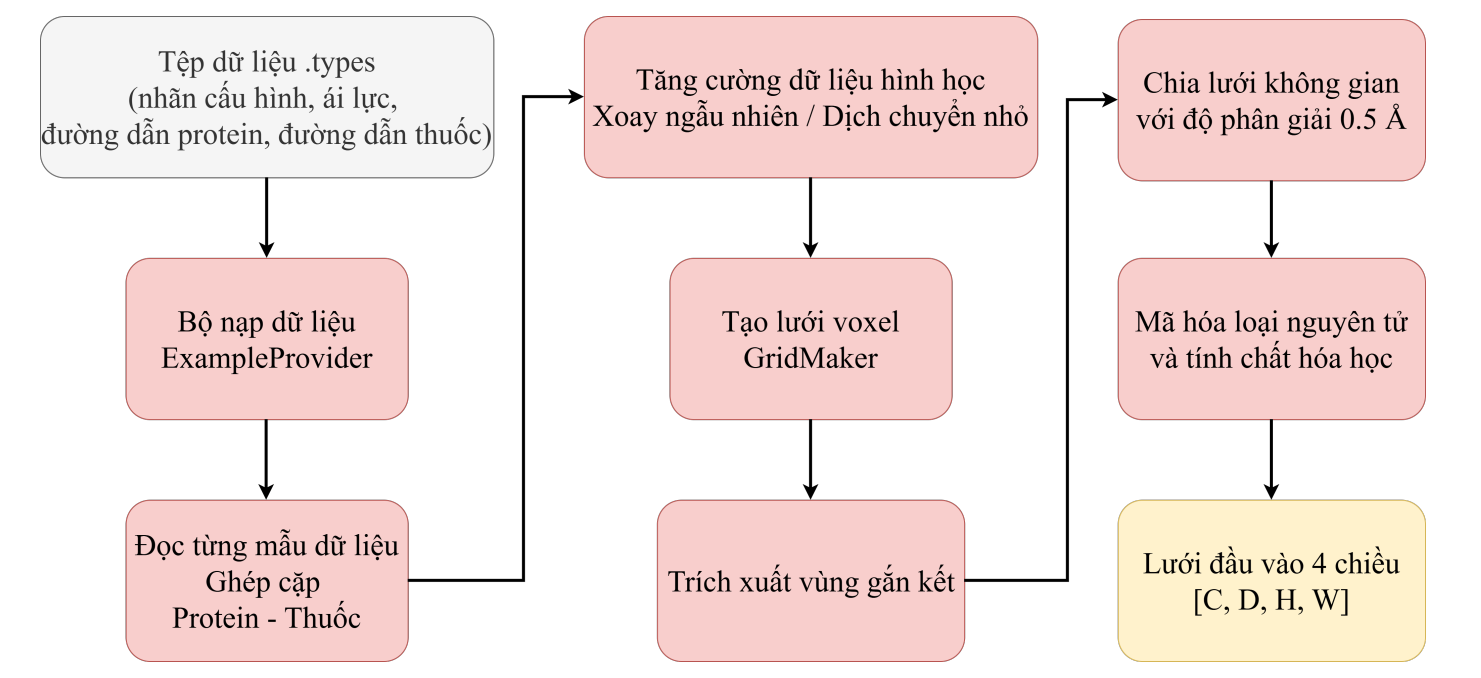
\includegraphics[width=0.5\textwidth]{figures/preprocessing.png}
    \caption{Quy trình tiền xử lý và tạo lưới voxel cho dữ liệu phức hợp protein -- phối tử.}
    \label{fig:preprocessing}
\end{figure}

Kết quả đầu ra của quy trình này là một lưới voxel có kích thước $48 \times 48 \times 48$, trong đó mỗi voxel được biểu diễn bởi 28 kênh đặc trưng mã hóa loại nguyên tử theo lược đồ atom-typing chuẩn của GNINA/libmolgrid (14 kênh cho protein, 14 kênh cho phối tử).

\begin{figure*}[t]
    \centering
    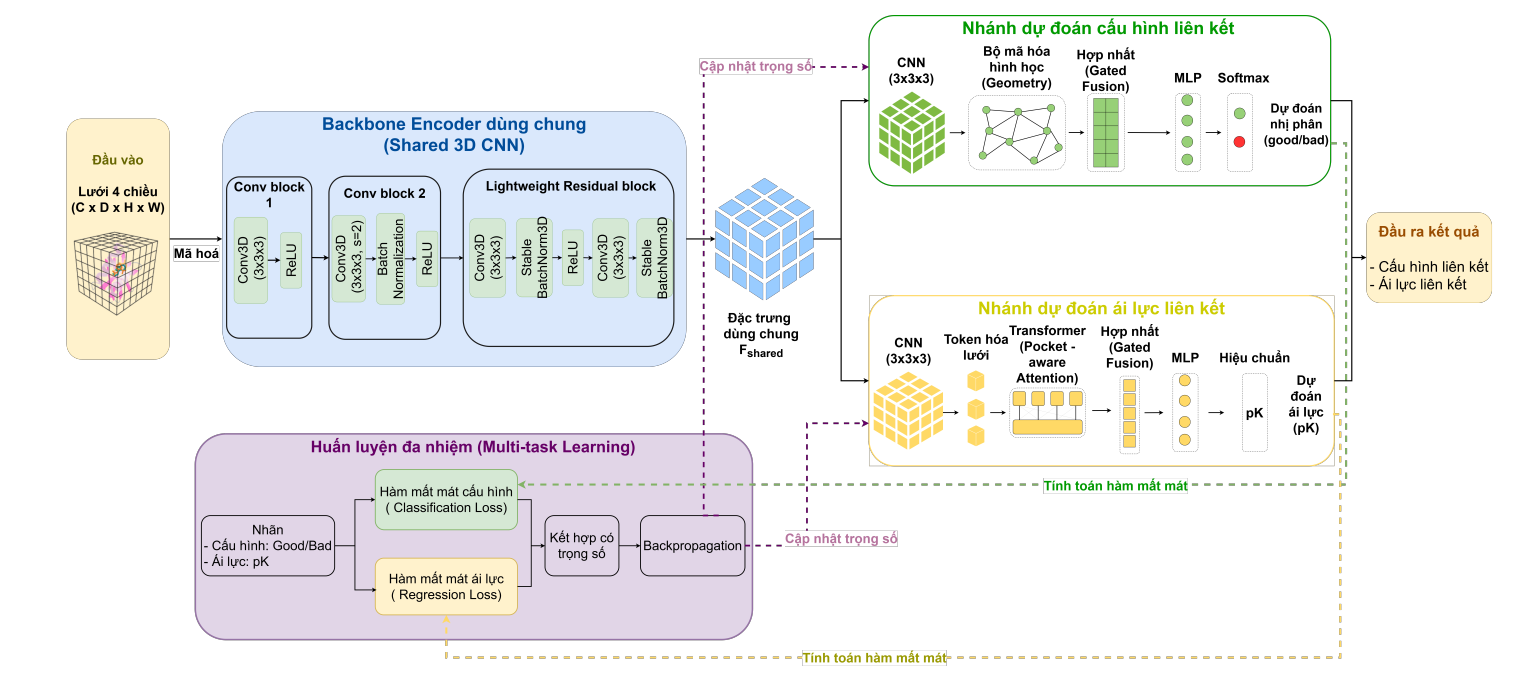
\includegraphics[width=0.9\textwidth]{figures/architecture.png}
    \caption{Tổng quan kiến trúc mô hình học đa nhiệm GeoFormerDock.}
    \label{fig:overall_architecture}
\end{figure*}

Mỗi mẫu mang hai loại nhãn riêng biệt: nhãn tư thế nhị phân $y_{pose} \in \{0,1\}$ (tốt/xấu) và giá trị ái lực $y_{aff} \in \mathbb{R}$. Nhãn $y_{pose}$ được xác định độc lập theo ngưỡng RMSD $\le 2$Å so với cấu trúc tham chiếu (cột RMSD trong tệp \texttt{.types}, quy ước gốc của CrossDocked2020/GNINA), với tỉ lệ dương thực tế là 12.4\% trên tập huấn luyện và 13.5\% trên tập kiểm tra. Theo quy ước của bộ dữ liệu, $y_{aff} > 0$ ứng với mẫu có ái lực thực nghiệm (đồng thời $y_{pose}=1$), còn $y_{aff} \le 0$ ứng với decoy; hai nhãn này không được dùng lẫn cho nhau ở bất kỳ bước huấn luyện/đánh giá nào - nhánh tư thế luôn dùng $y_{pose}$, nhánh ái lực luôn lọc theo dấu của $y_{aff}$ (xem mục hàm mất mát ái lực). Việc $y_{pose}=1$ luôn trùng với $y_{aff}>0$ không phải do gán nhãn chéo giữa hai tác vụ, mà do quy ước dấu: giá trị ái lực gốc chỉ giữ dương cho tư thế đúng (RMSD thấp) của phối tử thật và bị đảo dấu cho các tư thế/decoy còn lại - cùng một phức hợp có thể có cả tư thế tốt và xấu với cùng độ lớn ái lực nhưng khác dấu. Giá trị $y_{aff}$ (trên tập con $y_{aff}>0$) được chuẩn hóa theo phương pháp z-score trước khi đưa vào huấn luyện: $z = (y_{aff} - \mu)/\sigma$, với $\mu, \sigma$ ước lượng trên các nhãn ái lực dương của tập huấn luyện. Mạng được huấn luyện hoàn toàn trên thang chuẩn hóa này; khi đánh giá, dự đoán được đưa trở lại thang pK gốc trước khi tính các chỉ số.

\subsection{Kiến trúc GeoFormerDock}
GeoFormerDock được thiết kế theo nguyên lý học đa nhiệm~\cite{caruana1997multitask}, nhận đầu vào là lưới voxel và sử dụng một khối trích xuất đặc trưng dùng chung trước khi phân tách thành hai nhánh chuyên biệt để đánh giá tư thế và ái lực. Tổng quan kiến trúc của mô hình đề xuất được minh họa trong Hình \ref{fig:overall_architecture}, bao gồm mạng cơ sở dùng chung và hai nhánh học chuyên biệt được tối ưu hóa đồng thời.

\subsubsection{Khối trích xuất đặc trưng dùng chung}
Lưới voxel đi qua hai khối tích chập ba chiều duy trì tính tương biến theo phép tịnh tiến (translation equivariance)~\cite{ragoza2017protein}: khối thứ nhất dùng bộ lọc $3 \times 3 \times 3$ (bước trượt $s=1$, đệm $p=1$, 28$\to$32 kênh), khối thứ hai dùng bộ lọc $3 \times 3 \times 3$ (bước trượt $s=2$, 32$\to$48 kênh) để giảm chiều không gian, tiếp theo là một khối kết nối tắt dạng nhẹ~\cite{he2016deep} (hai lớp tích chập ba chiều kết hợp chuẩn hóa lô, một đường nối tắt tích chập $1 \times 1$ để khớp số kênh, và một lớp phi tuyến ReLU sau phép cộng), cho ra $F_{shared} \in \mathbb{R}^{64 \times 24 \times 24 \times 24}$, đóng vai trò cung cấp ngữ cảnh chung cho cả hai nhiệm vụ phía sau (xem tổng quan trong Hình \ref{fig:overall_architecture}).

\subsubsection{Nhánh phân loại tư thế gắn kết}
Nhánh này giải quyết bài toán phân loại tư thế bằng cách hợp nhất thông tin từ hai luồng: đặc trưng cục bộ và đặc trưng hình học.
Đối với luồng cục bộ, $F_{shared}$ đi qua khối tích chập cục bộ (hai lớp Conv3D $3\times3\times3$ xen một phép max-pooling $2\times2\times2$, giảm lưới không gian từ $24^3$ xuống $12^3$) để tạo ra $F_{pose}^{(1)} \in \mathbb{R}^{64\times12\times12\times12}$, sau đó được rút trích thông qua phép gom cụm trung bình toàn cục và một mạng nơ-ron truyền thẳng để tạo ra vector $h_{local}$.
Song song đó, luồng hình học chọn ra $K=12$ voxel có chuẩn kênh lớn nhất trên chính $F_{pose}^{(1)}$ làm các điểm trọng yếu (pseudo-atom), thu được tọa độ chuẩn hóa $p_i \in [-1,1]^3$ trên lưới cục bộ (\emph{không} phải đơn vị \AA) cùng vector đặc trưng kênh $a_i$ tương ứng. Khoảng cách Euclid $d_{ij} = ||p_i - p_j||_2$ giữa các cặp điểm được mã hóa qua $M=16$ hàm cơ sở xuyên tâm (tâm và bề rộng là tham số học được):
\begin{equation}
    \psi_{ij}^{(m)} = \exp\left(-\frac{(d_{ij} - \mu_m)^2}{2\sigma_m^2}\right)
    \label{eq:rbf}
\end{equation}
Đặc trưng kênh trung bình và ma trận RBF trung bình theo cặp được nối và chiếu qua một lớp truyền thẳng để tạo ra vector hình học $h_{geo}$.

Hai luồng thông tin được hợp nhất thông qua cơ chế cổng thích nghi:
\begin{equation}
    h_{fuse} = g \odot h_{local} + (1 - g) \odot h_{geo}
    \label{eq:fusion_pose}
\end{equation}
\newpage
Sơ đồ luồng xử lý và cơ chế hợp nhất đặc trưng giữa tuyến cục bộ và tuyến hình học được mô tả trong Hình \ref{fig:pose_branch}.

\begin{figure}[H]
    \centering
    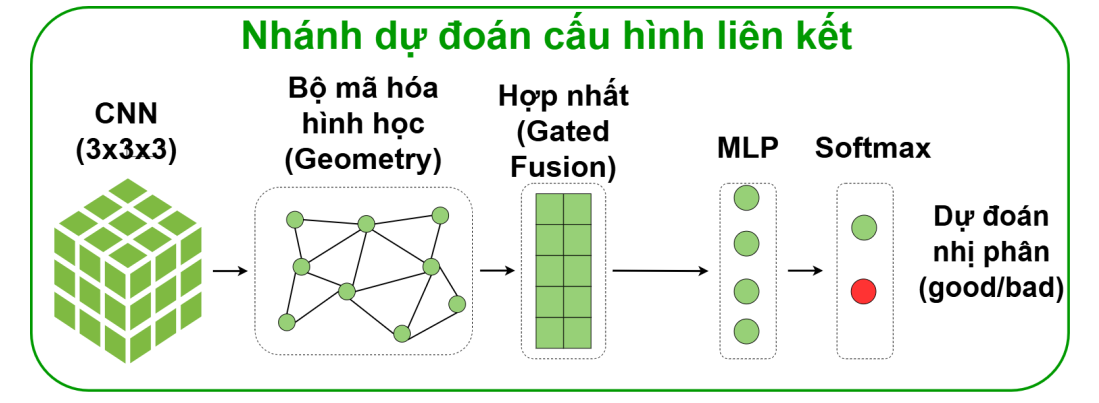
\includegraphics[width=0.5\textwidth]{figures/pose_branch.png}
    \caption{Kiến trúc nhánh phân loại tư thế gắn kết.}
    \label{fig:pose_branch}
\end{figure}

Kết quả cuối cùng đi qua lớp nơ-ron truyền thẳng và hàm softmax để đưa ra dự đoán nhị phân. Quá trình huấn luyện nhánh này sử dụng hàm mất mát tiêu điểm~\cite{lin2017focal} nhằm xử lý dữ liệu mất cân bằng, với xác suất dự đoán của lớp đúng $p_t$, hệ số tập trung $\gamma = 2.0$ giảm mức độ phạt từ mẫu dễ, trọng số cân bằng $\alpha_t = \alpha = 0.75$ nếu $y_i=1$, $\alpha_t = 1-\alpha$ nếu $y_i=0$ (ưu tiên lớp tư thế tốt):
\begin{equation}
    \ell_i = \alpha_t (1 - p_t)^\gamma \mathcal{L}_{NLL}^{(i)}
\end{equation}
Do dữ liệu mất cân bằng nghiêm trọng giữa hai lớp, tổn thất được gộp bằng \emph{trung bình cân bằng theo lớp} thay vì trung bình đơn giản trên toàn batch:
\begin{equation}
    \mathcal{L}_{pose} = \frac{1}{2}\left(\operatorname*{mean}_{i:\,y_i=0} \ell_i \;+\; \operatorname*{mean}_{i:\,y_i=1} \ell_i\right)
    \label{eq:lpose}
\end{equation}
Đồng thời, trước khi tính $\mathcal{L}_{pose}$, một tập con 64 mẫu (32 tốt/32 xấu) được lấy mẫu lại có hoàn lại từ minibatch 1024 mẫu để duy trì tỉ lệ lớp cố định riêng cho hàm mất mát này. Đây là một yếu tố thuộc về thiết lập huấn luyện có ảnh hưởng trực tiếp tới Balanced Accuracy, cần được tách bạch khỏi đóng góp của kiến trúc mạng khi diễn giải kết quả.

\subsubsection{Nhánh dự đoán ái lực liên kết}
Nhiệm vụ hồi quy ái lực đòi hỏi mô hình nhận thức được bức tranh toàn cục của túi liên kết. Tương tự nhánh tư thế, đặc trưng chung được xử lý qua khối tích chập cục bộ (Conv3D xen max-pooling $2\times2\times2$, giảm $24^3$ xuống $12^3$) để sinh ra $F_{aff}^{(1)} \in \mathbb{R}^{64\times12\times12\times12}$. Từ tensor này, mô hình tạo ra vector $h_{global}$ và chuyển đổi thành ma trận token $T \in \mathbb{R}^{N \times 128}$ với $N = 27$ (lưới token $3\times3\times3$, tương ứng chia $F_{aff}^{(1)}$ thành các patch kích thước 4 trên lưới cục bộ $12^3$).

Ma trận token được đưa vào 2 khối Transformer~\cite{vaswani2017attention} liên tiếp (embedding dim 128, tỉ lệ mở rộng MLP nội bộ là 2, dropout 0.1), trong đó cơ chế thiên vị chú ý theo khoá được thực hiện bằng một cổng sigmoid sinh độ chệch chú ý từ nội dung của từng token khoá (key-saliency gating), áp dụng độc lập cho mỗi trong 4 head (chỉ số head được bỏ qua trong công thức dưới đây để gọn):
\begin{equation}
    H = \mathrm{softmax}\!\left(\frac{QK^\top}{\sqrt{d_h}} + B_{pocket}\right)V
    \label{eq:attention}
\end{equation}
Trong đó, mỗi phần tử $[i,j]$ của ma trận độ chệch $B_{pocket}$ cộng vào bên trong softmax ở Phương trình~\eqref{eq:attention} được tính riêng cho từng head từ token khóa $\mathbf{x}_j \in \mathbb{R}^{128}$ (sau LayerNorm), với $\mathbf{w}, b$ là tham số riêng của head đó:
\begin{equation}
    B_{pocket}[i,j] = \sigma\left(\mathbf{w}^\top \mathbf{x}_j + b\right)
    \label{eq:bpocket}
\end{equation}
Khác với các cơ chế thiên vị chú ý dựa trên khoảng cách không gian tường minh, $B_{pocket}$ ở đây là độ chệch chú ý được sinh bởi một cổng sigmoid từ \emph{nội dung} của token khóa $j$: nó không sử dụng bất kỳ tọa độ 3D nào, và chỉ phụ thuộc token khóa $j$ - độc lập với token truy vấn $i$ (do đó chỉ số $i$ trong $[i,j]$ chỉ thể hiện việc bias này được cộng vào mọi hàng $i$ của ma trận điểm số, không phải bias phụ thuộc cặp $(i,j)$ thật). Bối cảnh túi liên kết vì vậy chỉ ảnh hưởng đến $B_{pocket}$ một cách gián tiếp, thông qua việc mỗi token đã mang thông tin mật độ nguyên tử của vùng không gian nó phủ, chứ không qua ràng buộc hình học tường minh giữa các cặp token. Đặc trưng token sau đó được tổng hợp thành $h_{token}$.

\begin{figure}[H]
    \centering
    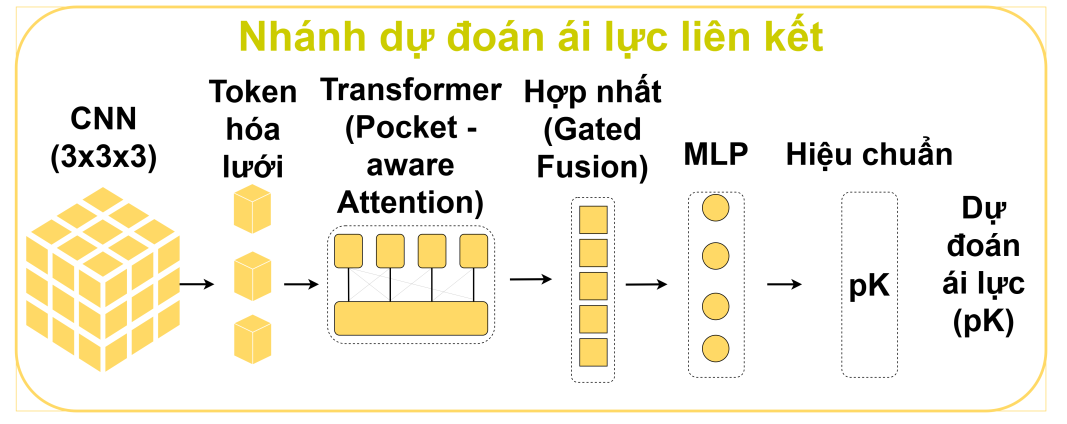
\includegraphics[width=0.5\textwidth]{figures/affinity_branch.png}
    \caption{Kiến trúc nhánh dự đoán ái lực liên kết.}
    \label{fig:affinity_branch}
\end{figure}

Quá trình trích xuất, token hóa và tích hợp cơ chế cổng thiên vị chú ý theo khóa của nhánh hồi quy ái lực được minh họa trong Hình \ref{fig:affinity_branch}.

Hai vector $h_{global}$ và $h_{token}$ được gộp cổng để tạo thành $h_{aff}$, sau đó đi qua một lớp MLP, và giới hạn biên bằng $\tau_{clamp}$ (Bảng~\ref{tab:hyperparams}) để cho ra $\hat{y}_{aff}$. Kiến trúc có kèm một phép hiệu chuẩn affine ($s \cdot \hat{y}_{aff} + b$) dành cho trường hợp huấn luyện trực tiếp trên thang pK gốc. Trong thiết lập thực nghiệm của bài báo (có chuẩn hóa z-score), $s=1, b=0$ được cố định nên không ảnh hưởng đến kết quả. Đây thuần túy là chi tiết cài đặt, không phải đóng góp kiến trúc.

Hàm mất mát của nhánh này là một tổ hợp đa mục tiêu nhằm điều tiết song song giá trị ái lực và quan hệ thứ tự:
\begin{equation}
\begin{aligned}
    \mathcal{L}_{aff} = \;&\lambda_{reg}\mathcal{L}_{reg} + \lambda_{rank}\mathcal{L}_{rank} \\
    &+ \lambda_{dist}\mathcal{L}_{dist} + \lambda_{anchor}\mathcal{L}_{anchor}
\end{aligned}
\label{eq:laff}
\end{equation}
Trong đó $\mathcal{L}_{reg}$ là hàm Huber ($\delta=1.0$), giúp hồi quy bền vững trước ngoại lai:
\begin{equation}
    \mathcal{L}_{reg}(y,\hat{y}) =
    \begin{cases}
    \frac{1}{2}(y-\hat{y})^2, & |y-\hat{y}| \le \delta \\
    \delta\!\left(|y-\hat{y}| - \frac{1}{2}\delta\right), & |y-\hat{y}| > \delta
    \end{cases}
    \label{eq:lreg}
\end{equation}
$\mathcal{L}_{rank}$ tối ưu thứ tự tương đối theo cặp mẫu ngẫu nhiên trong batch ($|\mathcal{P}|=128$, $\tau=1.0$):
\begin{equation}
    \begin{aligned}
        \mathcal{L}_{rank} &= \frac{1}{|\mathcal{P}|}\sum_{(i,j)\in\mathcal{P}} \mathrm{softplus}\Big[ -\mathrm{sign}(y_i-y_j) \\
        &\qquad\qquad\quad \cdot \mathrm{clamp}\!\left(\frac{\hat{y}_i-\hat{y}_j}{\tau},-5,5\right)\Big]
    \end{aligned}
    \label{eq:lrank}
\end{equation}
$\mathcal{L}_{dist}$ căn chỉnh kỳ vọng và độ lệch chuẩn giữa dự đoán và nhãn thật trong batch:
\begin{equation}
    \mathcal{L}_{dist} = |\mu_{\hat{y}} - \mu_y| + |\sigma_{\hat{y}} - \sigma_y|
    \label{eq:ldist}
\end{equation}
$\mathcal{L}_{anchor}$ dùng trung vị nhãn trong batch làm mỏ neo, tránh suy biến dự đoán:
\begin{equation}
    \mathcal{L}_{anchor} = \left|\hat{y} - \mathrm{median}(y)\right|
    \label{eq:lanchor}
\end{equation}

Cả bốn thành phần chỉ được tính trên tập mẫu có nhãn ái lực dương ($y_{aff} > 0$) - các mẫu decoy không đóng góp gradient cho nhánh ái lực.

\subsection{Tối ưu hóa đa nhiệm}
Hàm mất mát tổng thể được định nghĩa bằng sự kết hợp tuyến tính có trọng số:
\begin{equation}
    \mathcal{L}_{total} = w_{aff}\mathcal{L}_{aff} + w_{pose}\mathcal{L}_{pose}
    \label{eq:ltotal}
\end{equation}
Mạng được tối ưu hóa thông qua thuật toán AdamW~\cite{loshchilov2017decoupled} với tốc độ học $10^{-3}$ và hệ số điều chuẩn $10^{-2}$. Chiến lược điều chỉnh tốc độ học theo hàm cosin kết hợp cùng hai epoch khởi động được áp dụng nhằm ổn định quá trình lan truyền gradient trong giai đoạn đầu huấn luyện.

Mô hình được đánh giá sau mỗi 2 epoch; checkpoint tốt nhất được lựa chọn theo chỉ số tổng hợp $0.5 \cdot \text{C-index} + 0.5 \cdot \text{Balanced Accuracy}$, với early stopping nếu 25 lần đánh giá liên tiếp không cải thiện chỉ số này. Trong lần chạy báo cáo, chỉ số tổng hợp vẫn còn cải thiện tới gần cuối nên early stopping không kích hoạt trước khi đạt số epoch tối đa (100).


\begin{table}[H]
\centering
\caption{Hệ số hàm mất mát và siêu tham số}
\label{tab:hyperparams}
\footnotesize
\begin{tabular}{ll}
\hline
\textbf{Tham số} & \textbf{Giá trị} \\
\hline
$\tau_{clamp}$ (thang z-score) & 20 \\
$\lambda_{reg}, \lambda_{rank}, \lambda_{dist}, \lambda_{anchor}$ & 1.0, 0.05, 0.02, 0.01 \\
$w_{pose}, w_{aff}$ & 0.51, 0.15 \\
Batch size (chuẩn) & 1024 \\
\hline
\end{tabular}
\end{table}